\documentclass[12pt, oneside]{book}
\usepackage[utf8]{inputenc}
\usepackage{graphicx}
\usepackage[slovak]{babel}
\usepackage{todonotes}
\usepackage{url}
\usepackage{listings}
\usepackage{longtable}
\usepackage{pdflscape}
\usepackage{graphicx}
\usepackage{indentfirst}
\linespread{1.3}
\usepackage{chngcntr}
\counterwithout{footnote}{chapter}

\lstdefinestyle{customBash}{
  belowcaptionskip=1\baselineskip,
  breaklines=true,
  frame=L,
  xleftmargin=\parindent,
  language=bash,
  showstringspaces=false,
  basicstyle=\footnotesize\ttfamily,
  keywordstyle=\bfseries\color{green!40!black},
  commentstyle=\itshape\color{purple!40!black},
  identifierstyle=\color{blue},
  stringstyle=\color{red},
}

\lstdefinestyle{customC}{
  belowcaptionskip=1\baselineskip,
  breaklines=true,
  frame=L,
  xleftmargin=\parindent,
  language=c,
  showstringspaces=false,
  basicstyle=\footnotesize\ttfamily,
  keywordstyle=\bfseries\color{green!40!black},
  commentstyle=\itshape\color{purple!40!black},
  identifierstyle=\color{blue},
  stringstyle=\color{red},
}

\colorlet{punct}{red!60!black}
\definecolor{background}{HTML}{EEEEEE}
\definecolor{delim}{RGB}{20,105,176}
\colorlet{numb}{magenta!60!black}

\lstdefinelanguage{json}{
    basicstyle=\normalfont\ttfamily,
    numbers=left,
    numberstyle=\scriptsize,
    stepnumber=1,
    numbersep=8pt,
    showstringspaces=false,
    breaklines=true,
    frame=lines,
    backgroundcolor=\color{background},
    literate=
     *{0}{{{\color{numb}0}}}{1}
      {1}{{{\color{numb}1}}}{1}
      {2}{{{\color{numb}2}}}{1}
      {3}{{{\color{numb}3}}}{1}
      {4}{{{\color{numb}4}}}{1}
      {5}{{{\color{numb}5}}}{1}
      {6}{{{\color{numb}6}}}{1}
      {7}{{{\color{numb}7}}}{1}
      {8}{{{\color{numb}8}}}{1}
      {9}{{{\color{numb}9}}}{1}
      {:}{{{\color{punct}{:}}}}{1}
      {,}{{{\color{punct}{,}}}}{1}
      {\{}{{{\color{delim}{\{}}}}{1}
      {\}}{{{\color{delim}{\}}}}}{1}
      {[}{{{\color{delim}{[}}}}{1}
      {]}{{{\color{delim}{]}}}}{1},
}


\setcounter{secnumdepth}{3}
\setcounter{tocdepth}{3}

% -------------------
% --- Definicia zakladnych pommov
% -------------------
\def\*{{\bf FIXME: }}
\def\mfyear{2015}
\def\mftitle{Tvorba edukačného softvéru založeného na projekte Karel}
\def\mfthesistype{záverečná práca}
\def\mfauthor{Tomáš Kubla}
\def\mfadvisor{doc. PaedDr. Monika Tomcsányiová, PhD.}
\def\mfplacedate{Bratislava, \mfyear}
\def\odbor{2508 Informatika ??? } %aj cislo odboru je povinne a je to podla katedry/odboru, na ktorom je autor
\def\program{ Informatika ??? }
\def\stredisko{ Katedra základov a vyučovania Informatiky }

\begin{document}     

% -------------------
% --- Obalka ------
% -------------------
\thispagestyle{empty}
\noindent

\begin{minipage}{0.95\textwidth}
\begin{center}
\sc  
\large
\vspace*{0.3cm} Univerzita Komenského v Bratislave\\
\vspace*{0.3cm} Fakulta matematiky, fyziky a informatiky\\
\end{center}
\end{minipage}

\vfill

\begin{minipage}{1.1\textwidth}
\begin{flushright}
\bigskip\bigskip
% tusim mam nadstandardne dlhy nazov :)
%\centerline{\sc\LARGE\mftitle}
\begin{center}
\sc\LARGE\mftitle
\end{center}
\bigskip
\centerline{\sc\mfthesistype}

\bigskip\bigskip\bigskip\bigskip
\end{flushright}
\end{minipage}
\vfill

\noindent \mfyear\\
\indent\mfauthor

\eject % EOP i
% --- koniec obalky ----

% -------------------
% --- Titulný list
% -------------------

\thispagestyle{empty}
\noindent

\begin{minipage}{0.95\textwidth}
\begin{center}
\sc  
\large
\vspace*{0.3cm} Univerzita Komenského v Bratislave\\
\vspace*{0.3cm} Fakulta matematiky, fyziky a informatiky\\
\end{center}
\end{minipage}

\vfill

\begin{minipage}{1.1\textwidth}
\begin{flushright}
\bigskip\bigskip
% tusim mam nadstandardne dlhy nazov :)
%\centerline{\sc\LARGE\mftitle}
\begin{center}
\sc\LARGE\mftitle
\end{center}
\bigskip
\centerline{\sc\mfthesistype}
\end{flushright}

\bigskip
\vspace{3cm}
\bigskip
\begin{tabular}{ll}
Študijný program: & \program \\
Študijný odbor: & \odbor \\
Školiace pracovisko: & \stredisko \\
Školiteľ: & \mfadvisor \\
\end{tabular}

\end{minipage}
\vfill

\noindent \mfplacedate\\
\indent\mfauthor

\eject % EOP i


% --- Koniec titulnej strany


% -------------------
% --- Naskenovane Zadanie
% -------------------
% v tlačenej verzii s podpismi zainteresovaných osôb.
% v elektronickej verzii sa zverejňuje zadanie bez podpisov zainteresovaných osôb.

\newpage 
\thispagestyle{empty}
\hspace{-3cm}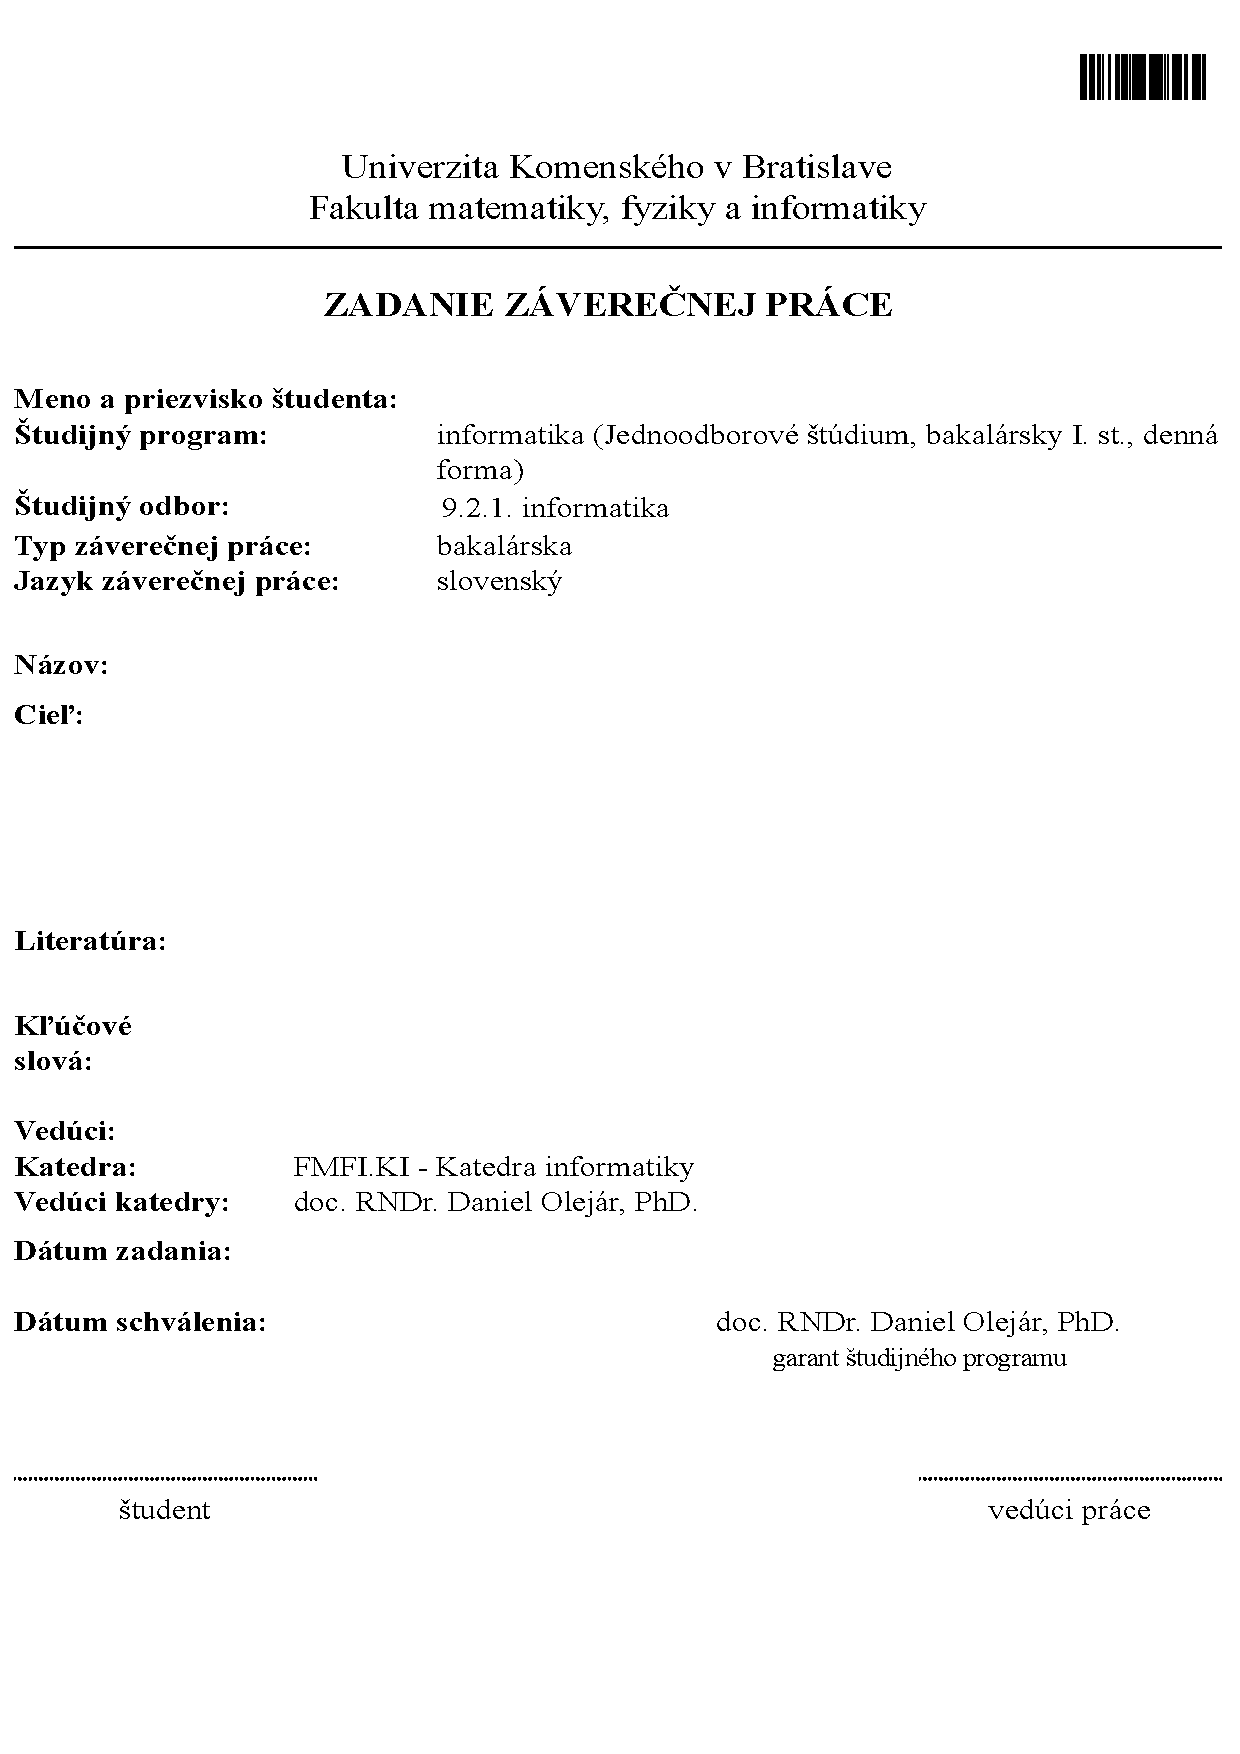
\includegraphics[width=1.4\textwidth]{images/zadanie.pdf}
%\hspace{-1cm}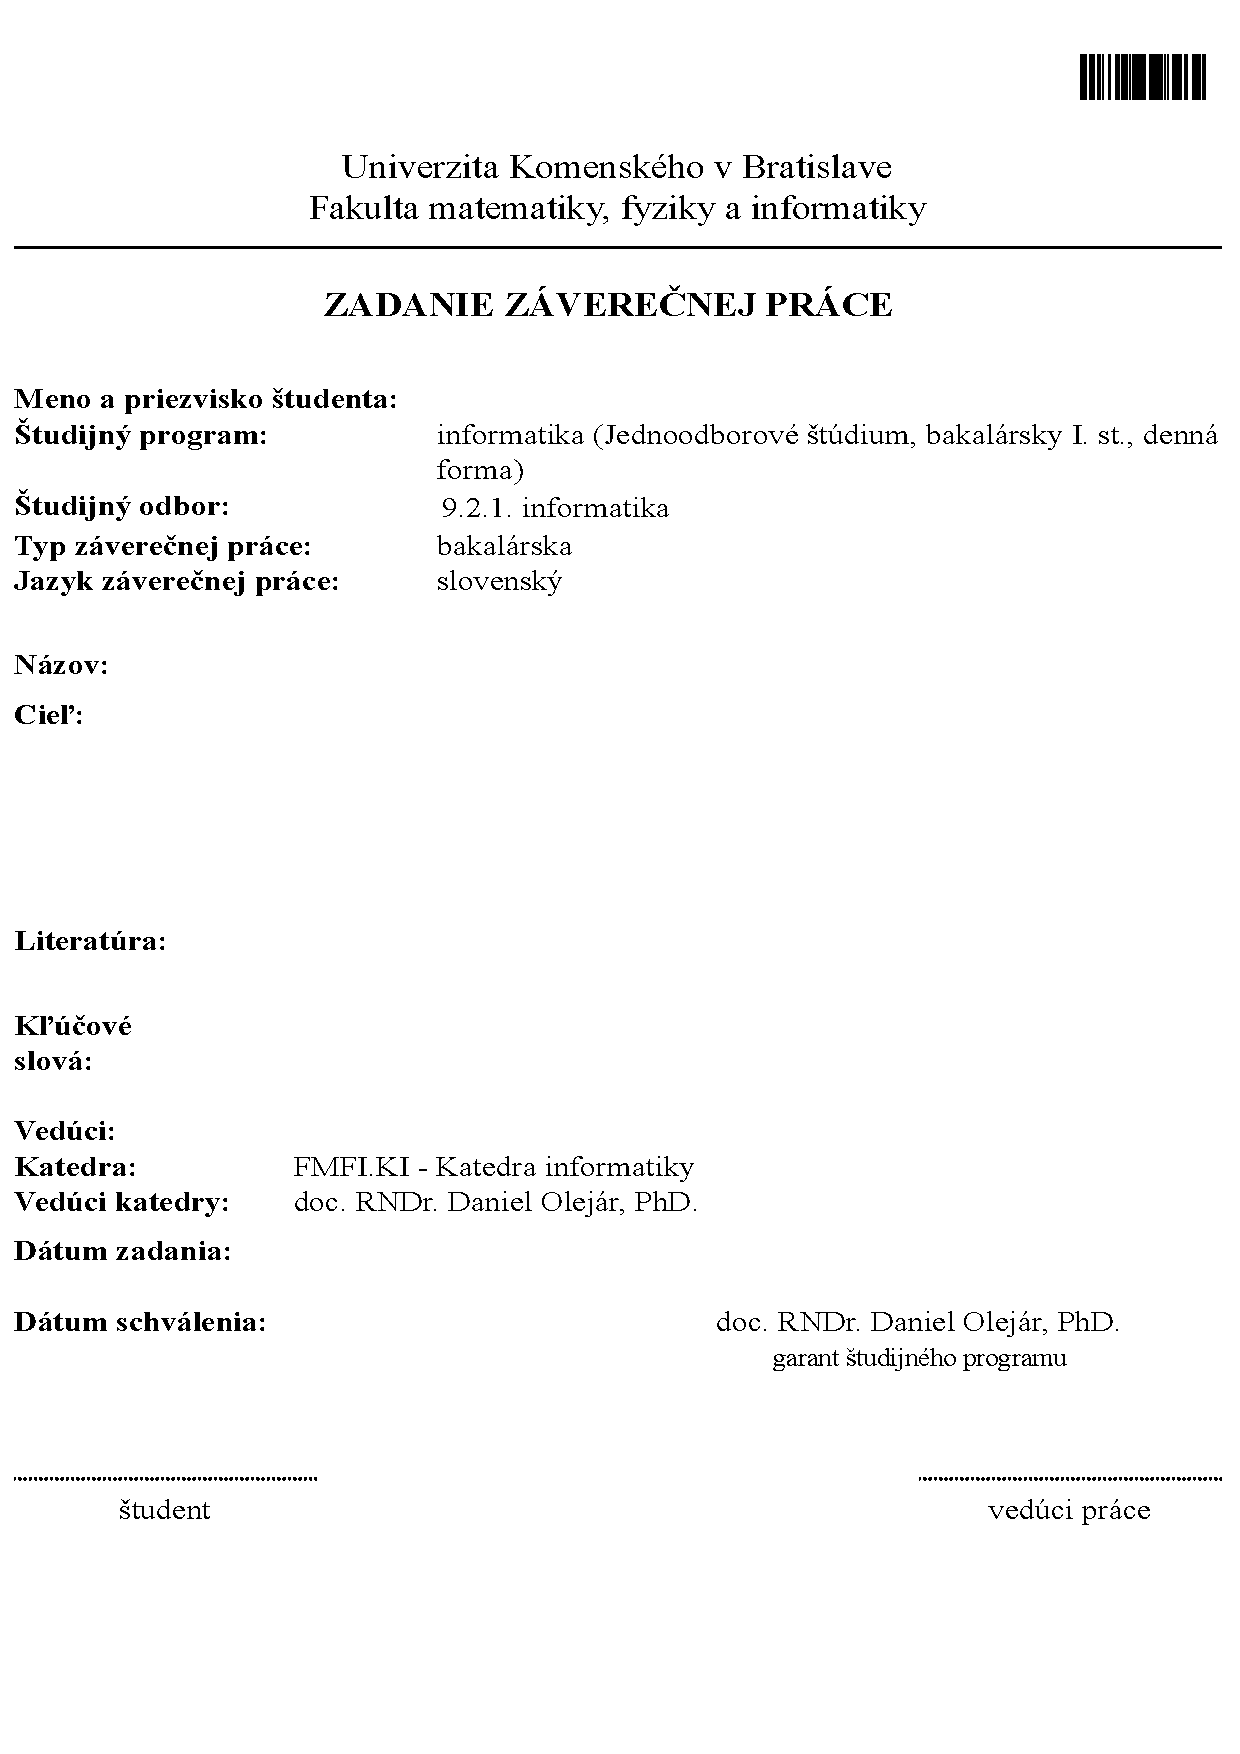
\includegraphics[width=1.2\textwidth]{images/zadanie.pdf}

% --- Koniec zadania

\frontmatter

% -------------------
%   Poďakovanie - nepovinné
% -------------------
\newpage 
\thispagestyle{empty}

\vfill
\huge{Poďakovanie}
%{\bf Poďakovanie:}
\normalsize
\newline
\todo{podakovanie}
%Chcel by som sa poďakovať RNDr. Jaroslavovi Janáčkovi PhD. za odbornú pomoc v oblasti počítačových sietí a za usmernenie pri tvorbe práce.
%Ďalej by som sa rád poďakoval všetkým ľuďom a inštitúciam, ktoré mi dovolili použiť ich infraštruktúru a servre na nasadenie honeypot-ov a za to, že som tieto dáta mohol použiť v analytickej a testovacej časti bakalársnej práce.
%Tiež by som sa chcel poďakovať svojej rodine a priateľke, ktorí ma podporovali počas celého štúdia.

% --- Koniec poďakovania

% -------------------
%   Abstrankt - Slovensky
% -------------------
\newpage 
\thispagestyle{empty}

\huge{Abstrakt}
\normalsize
\newline
\todo{abstrakt}
%Cieľom bakalárskej práce bolo vytvoriť honeypot na zber prihlasovacích údajov v bežne používaných službách.
%V prvej kapitole popisujeme pojem honeypot, jeho kategorizáciu a vysvetľujeme najčastejšie používanú sieťovú architekúru pri práci s honeypot-mi.
%Ďalej uvádzame popis všetkých technológií použitých pri tvorbe honeypot-u a jeho implementačné detaily.
%Taktiež navrhujeme rôzne postupy, ktorých uplatnením by mohlo dôjsť ku skvalitneniu nazberaných dát a k zvýšeniu ich počtu.
%Následne analyzujeme dáta nazberané naším honeypot-om.
%Uvádzame štatistiky a rôzne výsledky vyplývajúce z nazberaných údajov.
%V zá\-ve\-reč\-nej časti práce prezentujeme metódu, ktorou sme overovali, či existujúci informačný systém nie je zraniteľný na slovníkový útok nami zozberanými heslami.
%Prácou sme potvrdili, že klásť dôraz na informačnú bezpečnosť patrí k neodmysliteľným faktorom v súčasnom svete.
\\
\\
{\bf Kľúčové slová:} 
% --- Koniec Abstrakt - Slovensky


% -------------------
% --- Abstrakt - Anglicky 
% -------------------
\newpage 
\thispagestyle{empty}

\huge{Abstract}
\normalsize
\newline

\todo{abstract}
\\
\\
{\bf Keywords:} 

% --- Koniec Abstrakt - Anglicky

% -------------------
% --- Predhovor ?????
% -------------------
%\newpage 
%\thispagestyle{empty}
%
%\huge{Predhovor}
%\normalsize
%\newline
%Predhovor je všeobecná informácia o práci, obsahuje hlavnú charakteristiku práce 
%a okolnosti jej vzniku. Autor zdôvodní výber témy, stručne informuje o cieľoch 
%a význame práce, spomenie domáci a zahraničný kontext, komu je práca určená, 
%použité metódy, stav poznania; autor stručne charakterizuje svoj prístup a svoje 
%hľadisko. 
%
% --- Koniec Predhovor


% -------------------
% --- Obsah
% -------------------

\newpage 
\tableofcontents

% ---  Koniec Obsahu

% -------------------
% --- Zoznamy tabuliek, obrázkov
% -------------------

%\newpage 

%\listoffigures

% ---  Koniec Zoznamov

\mainmatter

\chapter*{Úvod}
\addcontentsline{toc}{chapter}{Úvod}



\chapter{PRACA}


\chapter*{Záver}
\addcontentsline{toc}{chapter}{Záver}



% -------------------
% --- Bibliografia
% -------------------


\newpage	

\backmatter

\thispagestyle{empty}
\nocite{*}
\clearpage

\bibliographystyle{plain}
%\bibliography{literatura} 
\addcontentsline{toc}{chapter}{Literatúra}

%Prípadne môžete napísať literatúru priamo tu
\begin{thebibliography}{5}
 
%\bibitem{hongkong} \uppercase{The Government of the Hong Kong Special Administrative Region}. Honeypot security.
%Feb. 2008 
%[cit. 2015-05-20].
%Dostupné na internete: \textless http://www.infosec.gov.hk/english/technical/files/honeypots.pdf\textgreater .


%\bibitem{technopedia} \uppercase{technopedia}. Honeypot.
%[cit. 2015-05-20].
%Dostupné na internete: \textless http://www.techopedia.com/definition/10278/honeypot\textgreater .

%\bibitem{pam} \uppercase{Open-source community}. Linux-PAM documentation.
%[cit. 2015-02-12].
%Dostupné na internete: \textless http://www.linux-pam.org/\textgreater .

%\bibitem{ksib} \uppercase{Daniel Olejár}. Krátky výkladový slovník termínov informačnej bezpečnosti. Verzia 1.0. Dec. 2011.

%\bibitem{oclhashcat} \uppercase{Jens Steube}. Oclhashcat documentation.
%[cit. 2015-05-26].
%Dostupné na internete: \textless http://hashcat.net/oclhashcat/\textgreater .

\end{thebibliography}

%---koniec Referencii

% -------------------
%--- Prilohy---
% -------------------

%Nepovinná časť prílohy obsahuje materiály, ktoré neboli zaradené priamo  do textu. Každá príloha sa začína na novej strane.
%Zoznam príloh je súčasťou obsahu.
%

\addcontentsline{toc}{chapter}{Prílohy}
\chapter*{Prílohy}
\thispagestyle{empty}


\newpage	

%\input AppendixA.tex
%
%\addcontentsline{toc}{chapter}{Appendix B}
%Zdrojovy kod2
%\input AppendixB.tex



\end{document}
